%comparatif avec le backInit
On peut voir sur le backlog ~\ref{bsp5} page~\pageref{bsp5} l'avancé du projet au sprint 5.
Nous avons rajouté des tâches, et des user-stories au fil du projet. En effet, nous avons eu de nouvelles idées à ajouter, et des fonctionnalités à écrire pour ne pas les oublier.
On peut aussi voir la justesse de nos estimations avec le temps réel passé sur chaque tâches.
Nous étions globalement dans les temps à chaque sprint, très peu de tâches ont été fini en retard.


\begin{figure}[h]
\caption{\label{bsp5} Backlog Sprint 5}
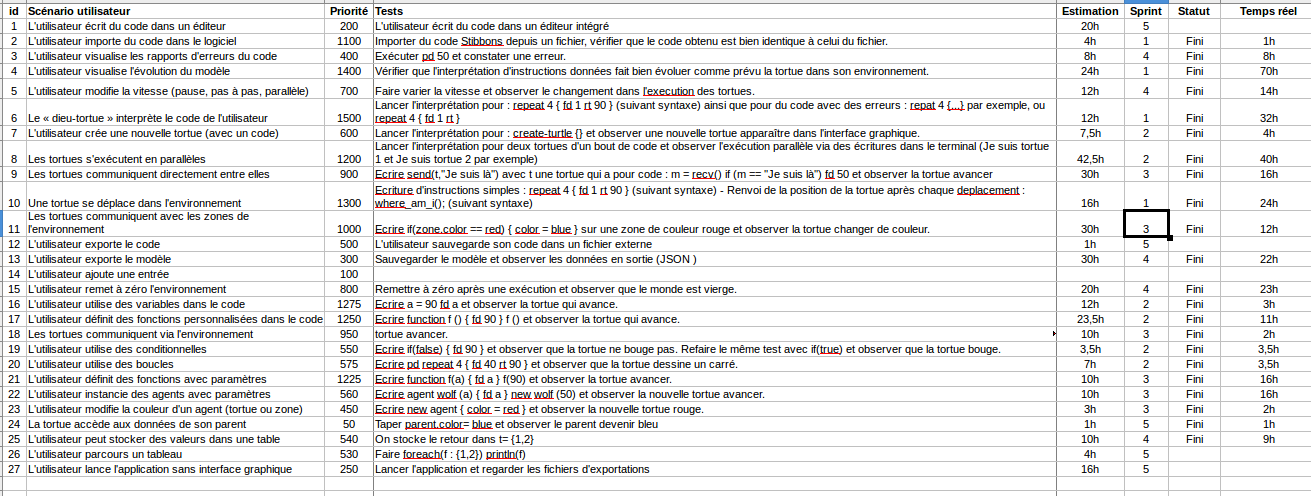
\includegraphics[scale=0.35]{doc/gestionProjet/backlogsp5.png}
\end{figure}
